\documentclass[1p]{elsarticle_modified}
%\bibliographystyle{elsarticle-num}

%\usepackage[colorlinks]{hyperref}
%\usepackage{abbrmath_seonhwa} %\Abb, \Ascr, \Acal ,\Abf, \Afrak
\usepackage{amsfonts}
\usepackage{amssymb}
\usepackage{amsmath}
\usepackage{amsthm}
\usepackage{scalefnt}
\usepackage{amsbsy}
\usepackage{kotex}
\usepackage{caption}
\usepackage{subfig}
\usepackage{color}
\usepackage{graphicx}
\usepackage{xcolor} %% white, black, red, green, blue, cyan, magenta, yellow
\usepackage{float}
\usepackage{setspace}
\usepackage{hyperref}

\usepackage{tikz}
\usetikzlibrary{arrows}

\usepackage{multirow}
\usepackage{array} % fixed length table
\usepackage{hhline}

%%%%%%%%%%%%%%%%%%%%%
\makeatletter
\renewcommand*\env@matrix[1][\arraystretch]{%
	\edef\arraystretch{#1}%
	\hskip -\arraycolsep
	\let\@ifnextchar\new@ifnextchar
	\array{*\c@MaxMatrixCols c}}
\makeatother %https://tex.stackexchange.com/questions/14071/how-can-i-increase-the-line-spacing-in-a-matrix
%%%%%%%%%%%%%%%

\usepackage[normalem]{ulem}

\newcommand{\msout}[1]{\ifmmode\text{\sout{\ensuremath{#1}}}\else\sout{#1}\fi}
%SOURCE: \msout is \stkout macro in https://tex.stackexchange.com/questions/20609/strikeout-in-math-mode

\newcommand{\cancel}[1]{
	\ifmmode
	{\color{red}\msout{#1}}
	\else
	{\color{red}\sout{#1}}
	\fi
}

\newcommand{\add}[1]{
	{\color{blue}\uwave{#1}}
}

\newcommand{\replace}[2]{
	\ifmmode
	{\color{red}\msout{#1}}{\color{blue}\uwave{#2}}
	\else
	{\color{red}\sout{#1}}{\color{blue}\uwave{#2}}
	\fi
}

\newcommand{\Sol}{\mathcal{S}} %segment
\newcommand{\D}{D} %diagram
\newcommand{\A}{\mathcal{A}} %arc


%%%%%%%%%%%%%%%%%%%%%%%%%%%%%5 test

\def\sl{\operatorname{\textup{SL}}(2,\Cbb)}
\def\psl{\operatorname{\textup{PSL}}(2,\Cbb)}
\def\quan{\mkern 1mu \triangleright \mkern 1mu}

\theoremstyle{definition}
\newtheorem{thm}{Theorem}[section]
\newtheorem{prop}[thm]{Proposition}
\newtheorem{lem}[thm]{Lemma}
\newtheorem{ques}[thm]{Question}
\newtheorem{cor}[thm]{Corollary}
\newtheorem{defn}[thm]{Definition}
\newtheorem{exam}[thm]{Example}
\newtheorem{rmk}[thm]{Remark}
\newtheorem{alg}[thm]{Algorithm}

\newcommand{\I}{\sqrt{-1}}
\begin{document}

%\begin{frontmatter}
%
%\title{Boundary parabolic representations of knots up to 8 crossings}
%
%%% Group authors per affiliation:
%\author{Yunhi Cho} 
%\address{Department of Mathematics, University of Seoul, Seoul, Korea}
%\ead{yhcho@uos.ac.kr}
%
%
%\author{Seonhwa Kim} %\fnref{s_kim}}
%\address{Center for Geometry and Physics, Institute for Basic Science, Pohang, 37673, Korea}
%\ead{ryeona17@ibs.re.kr}
%
%\author{Hyuk Kim}
%\address{Department of Mathematical Sciences, Seoul National University, Seoul 08826, Korea}
%\ead{hyukkim@snu.ac.kr}
%
%\author{Seokbeom Yoon}
%\address{Department of Mathematical Sciences, Seoul National University, Seoul, 08826,  Korea}
%\ead{sbyoon15@snu.ac.kr}
%
%\begin{abstract}
%We find all boundary parabolic representation of knots up to 8 crossings.
%
%\end{abstract}
%\begin{keyword}
%    \MSC[2010] 57M25 
%\end{keyword}
%
%\end{frontmatter}

%\linenumbers
%\tableofcontents
%
\newcommand\colored[1]{\textcolor{white}{\rule[-0.35ex]{0.8em}{1.4ex}}\kern-0.8em\color{red} #1}%
%\newcommand\colored[1]{\textcolor{white}{ #1}\kern-2.17ex	\textcolor{white}{ #1}\kern-1.81ex	\textcolor{white}{ #1}\kern-2.15ex\color{red}#1	}

{\Large $\underline{12a_{0276}~(K12a_{0276})}$}

\setlength{\tabcolsep}{10pt}
\renewcommand{\arraystretch}{1.6}
\vspace{1cm}\begin{tabular}{m{100pt}>{\centering\arraybackslash}m{274pt}}
\multirow{5}{120pt}{
	\centering
	\includegraphics[width=112pt]{../../../GIT/diagram.site/Diagrams/png/1077_12a_0276.png}\\
\ \ \ A knot diagram\footnotemark}&
\allowdisplaybreaks
\textbf{Linearized knot diagam} \\
\cline{2-2}
 &
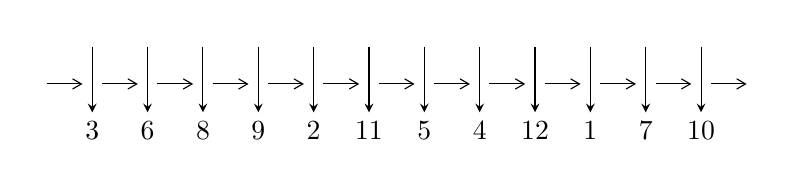
\begin{tikzpicture}[x=20pt, y=17pt]
	% nodes
	\node (C0) at (0, 0) {};
	\node (C1) at (1, 0) {};
	\node (C1U) at (1, +1) {};
	\node (C1D) at (1, -1) {3};

	\node (C2) at (2, 0) {};
	\node (C2U) at (2, +1) {};
	\node (C2D) at (2, -1) {6};

	\node (C3) at (3, 0) {};
	\node (C3U) at (3, +1) {};
	\node (C3D) at (3, -1) {8};

	\node (C4) at (4, 0) {};
	\node (C4U) at (4, +1) {};
	\node (C4D) at (4, -1) {9};

	\node (C5) at (5, 0) {};
	\node (C5U) at (5, +1) {};
	\node (C5D) at (5, -1) {2};

	\node (C6) at (6, 0) {};
	\node (C6U) at (6, +1) {};
	\node (C6D) at (6, -1) {11};

	\node (C7) at (7, 0) {};
	\node (C7U) at (7, +1) {};
	\node (C7D) at (7, -1) {5};

	\node (C8) at (8, 0) {};
	\node (C8U) at (8, +1) {};
	\node (C8D) at (8, -1) {4};

	\node (C9) at (9, 0) {};
	\node (C9U) at (9, +1) {};
	\node (C9D) at (9, -1) {12};

	\node (C10) at (10, 0) {};
	\node (C10U) at (10, +1) {};
	\node (C10D) at (10, -1) {1};

	\node (C11) at (11, 0) {};
	\node (C11U) at (11, +1) {};
	\node (C11D) at (11, -1) {7};

	\node (C12) at (12, 0) {};
	\node (C12U) at (12, +1) {};
	\node (C12D) at (12, -1) {10};
	\node (C13) at (13, 0) {};

	% arrows
	\draw[->,>={angle 60}]
	(C0) edge (C1) (C1) edge (C2) (C2) edge (C3) (C3) edge (C4) (C4) edge (C5) (C5) edge (C6) (C6) edge (C7) (C7) edge (C8) (C8) edge (C9) (C9) edge (C10) (C10) edge (C11) (C11) edge (C12) (C12) edge (C13) ;	\draw[->,>=stealth]
	(C1U) edge (C1D) (C2U) edge (C2D) (C3U) edge (C3D) (C4U) edge (C4D) (C5U) edge (C5D) (C6U) edge (C6D) (C7U) edge (C7D) (C8U) edge (C8D) (C9U) edge (C9D) (C10U) edge (C10D) (C11U) edge (C11D) (C12U) edge (C12D) ;
	\end{tikzpicture} \\
\hhline{~~} \\& 
\textbf{Solving Sequence} \\ \cline{2-2} 
 &
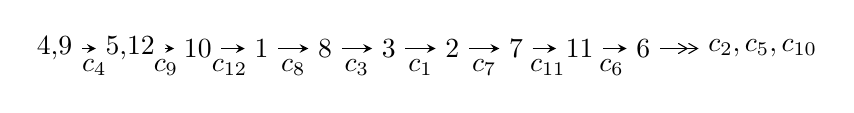
\begin{tikzpicture}[x=23pt, y=7pt]
	% node
	\node (A0) at (-1/8, 0) {4,9};
	\node (A1) at (17/16, 0) {5,12};
	\node (A2) at (17/8, 0) {10};
	\node (A3) at (25/8, 0) {1};
	\node (A4) at (33/8, 0) {8};
	\node (A5) at (41/8, 0) {3};
	\node (A6) at (49/8, 0) {2};
	\node (A7) at (57/8, 0) {7};
	\node (A8) at (65/8, 0) {11};
	\node (A9) at (73/8, 0) {6};
	\node (C1) at (1/2, -1) {$c_{4}$};
	\node (C2) at (13/8, -1) {$c_{9}$};
	\node (C3) at (21/8, -1) {$c_{12}$};
	\node (C4) at (29/8, -1) {$c_{8}$};
	\node (C5) at (37/8, -1) {$c_{3}$};
	\node (C6) at (45/8, -1) {$c_{1}$};
	\node (C7) at (53/8, -1) {$c_{7}$};
	\node (C8) at (61/8, -1) {$c_{11}$};
	\node (C9) at (69/8, -1) {$c_{6}$};
	\node (A10) at (11, 0) {$c_{2},c_{5},c_{10}$};

	% edge
	\draw[->,>=stealth]	
	(A0) edge (A1) (A1) edge (A2) (A2) edge (A3) (A3) edge (A4) (A4) edge (A5) (A5) edge (A6) (A6) edge (A7) (A7) edge (A8) (A8) edge (A9) ;
	\draw[->>,>={angle 60}]	
	(A9) edge (A10);
\end{tikzpicture} \\ 

\end{tabular} \\

\footnotetext{
The image of knot diagram is generated by the software ``\textbf{Draw programme}" developed by Andrew Bartholomew(\url{http://www.layer8.co.uk/maths/draw/index.htm\#Running-draw}), where we modified some parts for our purpose(\url{https://github.com/CATsTAILs/LinksPainter}).
}\phantom \\ \newline 
\centering \textbf{Ideals for irreducible components\footnotemark of $X_{\text{par}}$} 
 
\begin{align*}
I^u_{1}&=\langle 
3.34258\times10^{83} u^{91}-8.81488\times10^{83} u^{90}+\cdots+2.17711\times10^{84} b-2.38406\times10^{84},\\
\phantom{I^u_{1}}&\phantom{= \langle  }6.19627\times10^{83} u^{91}-1.41945\times10^{84} u^{90}+\cdots+2.17711\times10^{84} a-5.54877\times10^{83},\;u^{92}-2 u^{91}+\cdots+12 u+4\rangle \\
I^u_{2}&=\langle 
- u^7+u^6+2 u^5-3 u^4+2 u^2+b-2 u+2,\;u^7+u^6-3 u^5-2 u^4+3 u^3+a+2,\\
\phantom{I^u_{2}}&\phantom{= \langle  }u^8+u^7-3 u^6-2 u^5+3 u^4+2 u-1\rangle \\
I^u_{3}&=\langle 
a u+b-2 a- u-1,\;2 a^2- a u-1,\;u^2-2\rangle \\
\\
I^v_{1}&=\langle 
a,\;b+v+2,\;v^2+3 v+1\rangle \\
\end{align*}
\raggedright * 4 irreducible components of $\dim_{\mathbb{C}}=0$, with total 106 representations.\\
\footnotetext{All coefficients of polynomials are rational numbers. But the coefficients are sometimes approximated in decimal forms when there is not enough margin.}
\newpage
\renewcommand{\arraystretch}{1}
\centering \section*{I. $I^u_{1}= \langle 3.34\times10^{83} u^{91}-8.81\times10^{83} u^{90}+\cdots+2.18\times10^{84} b-2.38\times10^{84},\;6.20\times10^{83} u^{91}-1.42\times10^{84} u^{90}+\cdots+2.18\times10^{84} a-5.55\times10^{83},\;u^{92}-2 u^{91}+\cdots+12 u+4 \rangle$}
\flushleft \textbf{(i) Arc colorings}\\
\begin{tabular}{m{7pt} m{180pt} m{7pt} m{180pt} }
\flushright $a_{4}=$&$\begin{pmatrix}1\\0\end{pmatrix}$ \\
\flushright $a_{9}=$&$\begin{pmatrix}0\\u\end{pmatrix}$ \\
\flushright $a_{5}=$&$\begin{pmatrix}1\\u^2\end{pmatrix}$ \\
\flushright $a_{12}=$&$\begin{pmatrix}-0.284611 u^{91}+0.651991 u^{90}+\cdots-6.71279 u+0.254869\\-0.153533 u^{91}+0.404890 u^{90}+\cdots-1.63656 u+1.09506\end{pmatrix}$ \\
\flushright $a_{10}=$&$\begin{pmatrix}0.850284 u^{91}-1.32698 u^{90}+\cdots-1.86531 u+2.15950\\1.33947 u^{91}-1.25204 u^{90}+\cdots-11.3059 u-1.45062\end{pmatrix}$ \\
\flushright $a_{1}=$&$\begin{pmatrix}0.225091 u^{91}-0.817064 u^{90}+\cdots+8.33508 u+3.68616\\-0.466743 u^{91}-0.0372697 u^{90}+\cdots+5.80110 u+2.57471\end{pmatrix}$ \\
\flushright $a_{8}=$&$\begin{pmatrix}u\\u\end{pmatrix}$ \\
\flushright $a_{3}=$&$\begin{pmatrix}- u^2+1\\- u^2\end{pmatrix}$ \\
\flushright $a_{2}=$&$\begin{pmatrix}0.615650 u^{91}-1.09071 u^{90}+\cdots+3.61981 u+0.972754\\0.240176 u^{91}-0.305085 u^{90}+\cdots-3.12691 u+0.0205266\end{pmatrix}$ \\
\flushright $a_{7}=$&$\begin{pmatrix}- u^3+2 u\\- u^5+u^3+u\end{pmatrix}$ \\
\flushright $a_{11}=$&$\begin{pmatrix}-0.489371 u^{91}+0.911075 u^{90}+\cdots-4.78614 u+1.45037\\-0.651264 u^{91}+0.696436 u^{90}+\cdots+2.84926 u+2.67873\end{pmatrix}$ \\
\flushright $a_{6}=$&$\begin{pmatrix}-0.375474 u^{91}+0.785620 u^{90}+\cdots-6.74672 u-0.952228\\0.240176 u^{91}-0.305085 u^{90}+\cdots-3.12691 u+0.0205266\end{pmatrix}$\\&\end{tabular}
\flushleft \textbf{(ii) Obstruction class $= -1$}\\~\\
\flushleft \textbf{(iii) Cusp Shapes $= -3.63469 u^{91}+5.95903 u^{90}+\cdots+9.38857 u-43.1013$}\\~\\
\newpage\renewcommand{\arraystretch}{1}
\flushleft \textbf{(iv) u-Polynomials at the component}\newline \\
\begin{tabular}{m{50pt}|m{274pt}}
Crossings & \hspace{64pt}u-Polynomials at each crossing \\
\hline $$\begin{aligned}c_{1}\end{aligned}$$&$\begin{aligned}
&u^{92}+48 u^{91}+\cdots+1755 u+81
\end{aligned}$\\
\hline $$\begin{aligned}c_{2},c_{5}\end{aligned}$$&$\begin{aligned}
&u^{92}+4 u^{91}+\cdots-69 u-9
\end{aligned}$\\
\hline $$\begin{aligned}c_{3},c_{4},c_{8}\end{aligned}$$&$\begin{aligned}
&u^{92}+2 u^{91}+\cdots-12 u+4
\end{aligned}$\\
\hline $$\begin{aligned}c_{6},c_{11}\end{aligned}$$&$\begin{aligned}
&u^{92}-2 u^{91}+\cdots-1920 u+256
\end{aligned}$\\
\hline $$\begin{aligned}c_{7}\end{aligned}$$&$\begin{aligned}
&u^{92}-6 u^{91}+\cdots+6260 u+380
\end{aligned}$\\
\hline $$\begin{aligned}c_{9},c_{10},c_{12}\end{aligned}$$&$\begin{aligned}
&u^{92}-12 u^{91}+\cdots+6 u+1
\end{aligned}$\\
\hline
\end{tabular}\\~\\
\newpage\renewcommand{\arraystretch}{1}
\flushleft \textbf{(v) Riley Polynomials at the component}\newline \\
\begin{tabular}{m{50pt}|m{274pt}}
Crossings & \hspace{64pt}Riley Polynomials at each crossing \\
\hline $$\begin{aligned}c_{1}\end{aligned}$$&$\begin{aligned}
&y^{92}+72 y^{90}+\cdots-662499 y+6561
\end{aligned}$\\
\hline $$\begin{aligned}c_{2},c_{5}\end{aligned}$$&$\begin{aligned}
&y^{92}-48 y^{91}+\cdots-1755 y+81
\end{aligned}$\\
\hline $$\begin{aligned}c_{3},c_{4},c_{8}\end{aligned}$$&$\begin{aligned}
&y^{92}-86 y^{91}+\cdots-240 y+16
\end{aligned}$\\
\hline $$\begin{aligned}c_{6},c_{11}\end{aligned}$$&$\begin{aligned}
&y^{92}-60 y^{91}+\cdots-5947392 y+65536
\end{aligned}$\\
\hline $$\begin{aligned}c_{7}\end{aligned}$$&$\begin{aligned}
&y^{92}-14 y^{91}+\cdots-25869360 y+144400
\end{aligned}$\\
\hline $$\begin{aligned}c_{9},c_{10},c_{12}\end{aligned}$$&$\begin{aligned}
&y^{92}-92 y^{91}+\cdots+74 y+1
\end{aligned}$\\
\hline
\end{tabular}\\~\\
\newpage\flushleft \textbf{(vi) Complex Volumes and Cusp Shapes}
$$\begin{array}{c|c|c}  
\text{Solutions to }I^u_{1}& \I (\text{vol} + \sqrt{-1}CS) & \text{Cusp shape}\\
 \hline 
\begin{aligned}
u &= \phantom{-}0.969583 + 0.107648 I \\
a &= -0.003539 - 0.526904 I \\
b &= \phantom{-}0.459221 + 0.068074 I\end{aligned}
 & -0.513504 + 0.030259 I & \phantom{-0.000000 } 0 \\ \hline\begin{aligned}
u &= \phantom{-}0.969583 - 0.107648 I \\
a &= -0.003539 + 0.526904 I \\
b &= \phantom{-}0.459221 - 0.068074 I\end{aligned}
 & -0.513504 - 0.030259 I & \phantom{-0.000000 } 0 \\ \hline\begin{aligned}
u &= -1.03762\phantom{ +0.000000I} \\
a &= -1.39452\phantom{ +0.000000I} \\
b &= -0.0725617\phantom{ +0.000000I}\end{aligned}
 & -11.4153\phantom{ +0.000000I} & \phantom{-0.000000 } 0 \\ \hline\begin{aligned}
u &= -0.674626 + 0.619008 I \\
a &= -0.97265 - 1.31507 I \\
b &= -0.927957 + 0.305099 I\end{aligned}
 & -8.21616 - 7.69201 I & \phantom{-0.000000 } 0 \\ \hline\begin{aligned}
u &= -0.674626 - 0.619008 I \\
a &= -0.97265 + 1.31507 I \\
b &= -0.927957 - 0.305099 I\end{aligned}
 & -8.21616 + 7.69201 I & \phantom{-0.000000 } 0 \\ \hline\begin{aligned}
u &= \phantom{-}0.741480 + 0.527661 I \\
a &= \phantom{-}1.14534 - 1.08640 I \\
b &= \phantom{-}0.880522 + 0.160216 I\end{aligned}
 & -5.81043 + 2.35579 I & \phantom{-0.000000 } 0 \\ \hline\begin{aligned}
u &= \phantom{-}0.741480 - 0.527661 I \\
a &= \phantom{-}1.14534 + 1.08640 I \\
b &= \phantom{-}0.880522 - 0.160216 I\end{aligned}
 & -5.81043 - 2.35579 I & \phantom{-0.000000 } 0 \\ \hline\begin{aligned}
u &= -0.390955 + 0.781852 I \\
a &= -1.10343 - 1.35509 I \\
b &= -1.50467 + 0.09620 I\end{aligned}
 & -7.2837 + 12.4485 I & -16.5634 - 8.5018 I \\ \hline\begin{aligned}
u &= -0.390955 - 0.781852 I \\
a &= -1.10343 + 1.35509 I \\
b &= -1.50467 - 0.09620 I\end{aligned}
 & -7.2837 - 12.4485 I & -16.5634 + 8.5018 I \\ \hline\begin{aligned}
u &= \phantom{-}0.063829 + 0.858332 I \\
a &= \phantom{-}0.17179 - 1.48729 I \\
b &= \phantom{-}0.216749 - 0.221340 I\end{aligned}
 & -0.63733 - 3.04639 I & -16.3980 + 3.8542 I\\
 \hline 
 \end{array}$$\newpage$$\begin{array}{c|c|c}  
\text{Solutions to }I^u_{1}& \I (\text{vol} + \sqrt{-1}CS) & \text{Cusp shape}\\
 \hline 
\begin{aligned}
u &= \phantom{-}0.063829 - 0.858332 I \\
a &= \phantom{-}0.17179 + 1.48729 I \\
b &= \phantom{-}0.216749 + 0.221340 I\end{aligned}
 & -0.63733 + 3.04639 I & -16.3980 - 3.8542 I \\ \hline\begin{aligned}
u &= \phantom{-}0.330243 + 0.776749 I \\
a &= \phantom{-}0.97602 - 1.44162 I \\
b &= \phantom{-}1.296880 - 0.073620 I\end{aligned}
 & -4.46168 - 6.88858 I & -13.9256 + 5.1752 I \\ \hline\begin{aligned}
u &= \phantom{-}0.330243 - 0.776749 I \\
a &= \phantom{-}0.97602 + 1.44162 I \\
b &= \phantom{-}1.296880 + 0.073620 I\end{aligned}
 & -4.46168 + 6.88858 I & -13.9256 - 5.1752 I \\ \hline\begin{aligned}
u &= -1.180620 + 0.049140 I \\
a &= \phantom{-}0.905051 + 0.405129 I \\
b &= \phantom{-}1.71434 - 0.47461 I\end{aligned}
 & -4.02322 + 0.72103 I & \phantom{-0.000000 } 0 \\ \hline\begin{aligned}
u &= -1.180620 - 0.049140 I \\
a &= \phantom{-}0.905051 - 0.405129 I \\
b &= \phantom{-}1.71434 + 0.47461 I\end{aligned}
 & -4.02322 - 0.72103 I & \phantom{-0.000000 } 0 \\ \hline\begin{aligned}
u &= -0.341347 + 0.720746 I \\
a &= \phantom{-}1.198680 - 0.029660 I \\
b &= \phantom{-}0.788988 - 0.152649 I\end{aligned}
 & -1.23377 + 8.07113 I & -13.5538 - 8.5121 I \\ \hline\begin{aligned}
u &= -0.341347 - 0.720746 I \\
a &= \phantom{-}1.198680 + 0.029660 I \\
b &= \phantom{-}0.788988 + 0.152649 I\end{aligned}
 & -1.23377 - 8.07113 I & -13.5538 + 8.5121 I \\ \hline\begin{aligned}
u &= -1.184720 + 0.249629 I \\
a &= \phantom{-}0.146188 - 0.546688 I \\
b &= \phantom{-}0.0273490 + 0.0956059 I\end{aligned}
 & -0.85249 + 4.72720 I & \phantom{-0.000000 } 0 \\ \hline\begin{aligned}
u &= -1.184720 - 0.249629 I \\
a &= \phantom{-}0.146188 + 0.546688 I \\
b &= \phantom{-}0.0273490 - 0.0956059 I\end{aligned}
 & -0.85249 - 4.72720 I & \phantom{-0.000000 } 0 \\ \hline\begin{aligned}
u &= -0.616721 + 0.490885 I \\
a &= -0.221693 + 1.040660 I \\
b &= -0.229638 + 0.292595 I\end{aligned}
 & -2.26213 - 3.90874 I & -15.3859 + 3.7108 I\\
 \hline 
 \end{array}$$\newpage$$\begin{array}{c|c|c}  
\text{Solutions to }I^u_{1}& \I (\text{vol} + \sqrt{-1}CS) & \text{Cusp shape}\\
 \hline 
\begin{aligned}
u &= -0.616721 - 0.490885 I \\
a &= -0.221693 - 1.040660 I \\
b &= -0.229638 - 0.292595 I\end{aligned}
 & -2.26213 + 3.90874 I & -15.3859 - 3.7108 I \\ \hline\begin{aligned}
u &= \phantom{-}1.210350 + 0.144980 I \\
a &= -1.027120 - 0.175344 I \\
b &= -2.53696 + 0.78808 I\end{aligned}
 & -4.28970 - 3.40044 I & \phantom{-0.000000 } 0 \\ \hline\begin{aligned}
u &= \phantom{-}1.210350 - 0.144980 I \\
a &= -1.027120 + 0.175344 I \\
b &= -2.53696 - 0.78808 I\end{aligned}
 & -4.28970 + 3.40044 I & \phantom{-0.000000 } 0 \\ \hline\begin{aligned}
u &= \phantom{-}1.146230 + 0.420367 I \\
a &= \phantom{-}1.010760 - 0.337976 I \\
b &= \phantom{-}1.263380 - 0.483375 I\end{aligned}
 & -3.97193 - 1.52452 I & \phantom{-0.000000 } 0 \\ \hline\begin{aligned}
u &= \phantom{-}1.146230 - 0.420367 I \\
a &= \phantom{-}1.010760 + 0.337976 I \\
b &= \phantom{-}1.263380 + 0.483375 I\end{aligned}
 & -3.97193 + 1.52452 I & \phantom{-0.000000 } 0 \\ \hline\begin{aligned}
u &= \phantom{-}0.341585 + 0.668395 I \\
a &= -1.05640 + 1.61061 I \\
b &= -1.30954 - 0.55648 I\end{aligned}
 & -3.99403 - 5.59592 I & -15.4677 + 6.2129 I \\ \hline\begin{aligned}
u &= \phantom{-}0.341585 - 0.668395 I \\
a &= -1.05640 - 1.61061 I \\
b &= -1.30954 + 0.55648 I\end{aligned}
 & -3.99403 + 5.59592 I & -15.4677 - 6.2129 I \\ \hline\begin{aligned}
u &= \phantom{-}0.188441 + 0.708555 I \\
a &= \phantom{-}0.638248 - 0.300259 I \\
b &= \phantom{-}0.471116 + 0.361008 I\end{aligned}
 & \phantom{-}1.75825 - 3.49258 I & -7.18786 + 5.15359 I \\ \hline\begin{aligned}
u &= \phantom{-}0.188441 - 0.708555 I \\
a &= \phantom{-}0.638248 + 0.300259 I \\
b &= \phantom{-}0.471116 - 0.361008 I\end{aligned}
 & \phantom{-}1.75825 + 3.49258 I & -7.18786 - 5.15359 I \\ \hline\begin{aligned}
u &= -0.279771 + 0.668738 I \\
a &= -1.02400 - 1.79888 I \\
b &= -1.37269 - 0.62207 I\end{aligned}
 & -9.80694 + 2.97546 I & -17.9875 - 3.6008 I\\
 \hline 
 \end{array}$$\newpage$$\begin{array}{c|c|c}  
\text{Solutions to }I^u_{1}& \I (\text{vol} + \sqrt{-1}CS) & \text{Cusp shape}\\
 \hline 
\begin{aligned}
u &= -0.279771 - 0.668738 I \\
a &= -1.02400 + 1.79888 I \\
b &= -1.37269 + 0.62207 I\end{aligned}
 & -9.80694 - 2.97546 I & -17.9875 + 3.6008 I \\ \hline\begin{aligned}
u &= \phantom{-}0.252374 + 0.668121 I \\
a &= -1.118440 + 0.021493 I \\
b &= -0.759308 + 0.065796 I\end{aligned}
 & \phantom{-}1.14826 - 3.17312 I & -9.30715 + 5.02148 I \\ \hline\begin{aligned}
u &= \phantom{-}0.252374 - 0.668121 I \\
a &= -1.118440 - 0.021493 I \\
b &= -0.759308 - 0.065796 I\end{aligned}
 & \phantom{-}1.14826 + 3.17312 I & -9.30715 - 5.02148 I \\ \hline\begin{aligned}
u &= \phantom{-}1.273630 + 0.242181 I \\
a &= \phantom{-}0.285414 + 0.261261 I \\
b &= \phantom{-}1.316700 + 0.008357 I\end{aligned}
 & -1.34793 - 2.04566 I & \phantom{-0.000000 } 0 \\ \hline\begin{aligned}
u &= \phantom{-}1.273630 - 0.242181 I \\
a &= \phantom{-}0.285414 - 0.261261 I \\
b &= \phantom{-}1.316700 - 0.008357 I\end{aligned}
 & -1.34793 + 2.04566 I & \phantom{-0.000000 } 0 \\ \hline\begin{aligned}
u &= \phantom{-}0.508498 + 0.473897 I \\
a &= -1.32056 + 1.41639 I \\
b &= -1.73251 - 0.27223 I\end{aligned}
 & -4.75530 + 1.78277 I & -17.3380 + 0.3544 I \\ \hline\begin{aligned}
u &= \phantom{-}0.508498 - 0.473897 I \\
a &= -1.32056 - 1.41639 I \\
b &= -1.73251 + 0.27223 I\end{aligned}
 & -4.75530 - 1.78277 I & -17.3380 - 0.3544 I \\ \hline\begin{aligned}
u &= -0.300885 + 0.616253 I \\
a &= -0.35830 + 1.49912 I \\
b &= -0.158598 - 0.016331 I\end{aligned}
 & -2.55198 + 2.76644 I & -15.5409 - 4.4573 I \\ \hline\begin{aligned}
u &= -0.300885 - 0.616253 I \\
a &= -0.35830 - 1.49912 I \\
b &= -0.158598 + 0.016331 I\end{aligned}
 & -2.55198 - 2.76644 I & -15.5409 + 4.4573 I \\ \hline\begin{aligned}
u &= -0.030654 + 0.683608 I \\
a &= -0.780875 - 0.127083 I \\
b &= -0.481566 + 0.327235 I\end{aligned}
 & \phantom{-}2.66095 - 1.28667 I & -5.71389 + 2.78365 I\\
 \hline 
 \end{array}$$\newpage$$\begin{array}{c|c|c}  
\text{Solutions to }I^u_{1}& \I (\text{vol} + \sqrt{-1}CS) & \text{Cusp shape}\\
 \hline 
\begin{aligned}
u &= -0.030654 - 0.683608 I \\
a &= -0.780875 + 0.127083 I \\
b &= -0.481566 - 0.327235 I\end{aligned}
 & \phantom{-}2.66095 + 1.28667 I & -5.71389 - 2.78365 I \\ \hline\begin{aligned}
u &= \phantom{-}0.666845 + 0.068325 I \\
a &= -0.075581 + 0.622950 I \\
b &= \phantom{-}0.422885 + 0.072774 I\end{aligned}
 & -0.523648 - 0.094088 I & -11.87057 + 0.12396 I \\ \hline\begin{aligned}
u &= \phantom{-}0.666845 - 0.068325 I \\
a &= -0.075581 - 0.622950 I \\
b &= \phantom{-}0.422885 - 0.072774 I\end{aligned}
 & -0.523648 + 0.094088 I & -11.87057 - 0.12396 I \\ \hline\begin{aligned}
u &= -1.270790 + 0.395450 I \\
a &= -0.962888 - 0.190034 I \\
b &= -1.70094 - 0.74003 I\end{aligned}
 & -4.78582 + 7.53244 I & \phantom{-0.000000 } 0 \\ \hline\begin{aligned}
u &= -1.270790 - 0.395450 I \\
a &= -0.962888 + 0.190034 I \\
b &= -1.70094 + 0.74003 I\end{aligned}
 & -4.78582 - 7.53244 I & \phantom{-0.000000 } 0 \\ \hline\begin{aligned}
u &= -1.33936\phantom{ +0.000000I} \\
a &= -1.25475\phantom{ +0.000000I} \\
b &= -3.76057\phantom{ +0.000000I}\end{aligned}
 & -14.2652\phantom{ +0.000000I} & \phantom{-0.000000 } 0 \\ \hline\begin{aligned}
u &= -1.354420 + 0.050875 I \\
a &= -0.0211295 + 0.0997711 I \\
b &= -1.50291 - 0.41520 I\end{aligned}
 & -6.43271 + 0.08678 I & \phantom{-0.000000 } 0 \\ \hline\begin{aligned}
u &= -1.354420 - 0.050875 I \\
a &= -0.0211295 - 0.0997711 I \\
b &= -1.50291 + 0.41520 I\end{aligned}
 & -6.43271 - 0.08678 I & \phantom{-0.000000 } 0 \\ \hline\begin{aligned}
u &= -1.375350 + 0.176357 I \\
a &= \phantom{-}0.525875 + 0.521338 I \\
b &= \phantom{-}0.890304 + 0.387213 I\end{aligned}
 & -5.48308 + 1.43317 I & \phantom{-0.000000 } 0 \\ \hline\begin{aligned}
u &= -1.375350 - 0.176357 I \\
a &= \phantom{-}0.525875 - 0.521338 I \\
b &= \phantom{-}0.890304 - 0.387213 I\end{aligned}
 & -5.48308 - 1.43317 I & \phantom{-0.000000 } 0\\
 \hline 
 \end{array}$$\newpage$$\begin{array}{c|c|c}  
\text{Solutions to }I^u_{1}& \I (\text{vol} + \sqrt{-1}CS) & \text{Cusp shape}\\
 \hline 
\begin{aligned}
u &= -1.363580 + 0.289426 I \\
a &= -0.378679 + 0.156042 I \\
b &= -1.58342 + 0.01614 I\end{aligned}
 & -3.14548 + 7.11465 I & \phantom{-0.000000 } 0 \\ \hline\begin{aligned}
u &= -1.363580 - 0.289426 I \\
a &= -0.378679 - 0.156042 I \\
b &= -1.58342 - 0.01614 I\end{aligned}
 & -3.14548 - 7.11465 I & \phantom{-0.000000 } 0 \\ \hline\begin{aligned}
u &= -0.252729 + 0.545556 I \\
a &= \phantom{-}1.12490 + 1.80734 I \\
b &= \phantom{-}1.195530 - 0.220149 I\end{aligned}
 & -1.55180 + 1.30485 I & -10.68807 - 2.05814 I \\ \hline\begin{aligned}
u &= -0.252729 - 0.545556 I \\
a &= \phantom{-}1.12490 - 1.80734 I \\
b &= \phantom{-}1.195530 + 0.220149 I\end{aligned}
 & -1.55180 - 1.30485 I & -10.68807 + 2.05814 I \\ \hline\begin{aligned}
u &= \phantom{-}1.40328\phantom{ +0.000000I} \\
a &= -0.707097\phantom{ +0.000000I} \\
b &= \phantom{-}17.9866\phantom{ +0.000000I}\end{aligned}
 & -8.20346\phantom{ +0.000000I} & \phantom{-0.000000 } 0 \\ \hline\begin{aligned}
u &= \phantom{-}1.40268 + 0.21970 I \\
a &= -1.000470 + 0.047291 I \\
b &= -4.06076 + 1.13846 I\end{aligned}
 & -6.86940 - 4.15900 I & \phantom{-0.000000 } 0 \\ \hline\begin{aligned}
u &= \phantom{-}1.40268 - 0.21970 I \\
a &= -1.000470 - 0.047291 I \\
b &= -4.06076 - 1.13846 I\end{aligned}
 & -6.86940 + 4.15900 I & \phantom{-0.000000 } 0 \\ \hline\begin{aligned}
u &= -1.40166 + 0.25943 I \\
a &= \phantom{-}0.369957 - 0.538443 I \\
b &= \phantom{-}1.406840 - 0.025933 I\end{aligned}
 & -4.13348 + 6.54909 I & \phantom{-0.000000 } 0 \\ \hline\begin{aligned}
u &= -1.40166 - 0.25943 I \\
a &= \phantom{-}0.369957 + 0.538443 I \\
b &= \phantom{-}1.406840 + 0.025933 I\end{aligned}
 & -4.13348 - 6.54909 I & \phantom{-0.000000 } 0 \\ \hline\begin{aligned}
u &= \phantom{-}1.41699 + 0.18942 I \\
a &= -0.397552 - 0.451392 I \\
b &= -1.82800 + 0.67940 I\end{aligned}
 & -8.80343 - 2.85042 I & \phantom{-0.000000 } 0\\
 \hline 
 \end{array}$$\newpage$$\begin{array}{c|c|c}  
\text{Solutions to }I^u_{1}& \I (\text{vol} + \sqrt{-1}CS) & \text{Cusp shape}\\
 \hline 
\begin{aligned}
u &= \phantom{-}1.41699 - 0.18942 I \\
a &= -0.397552 + 0.451392 I \\
b &= -1.82800 - 0.67940 I\end{aligned}
 & -8.80343 + 2.85042 I & \phantom{-0.000000 } 0 \\ \hline\begin{aligned}
u &= \phantom{-}1.42092 + 0.16882 I \\
a &= \phantom{-}1.142530 - 0.249164 I \\
b &= \phantom{-}3.80818 - 0.16162 I\end{aligned}
 & -16.6231 - 2.4062 I & \phantom{-0.000000 } 0 \\ \hline\begin{aligned}
u &= \phantom{-}1.42092 - 0.16882 I \\
a &= \phantom{-}1.142530 + 0.249164 I \\
b &= \phantom{-}3.80818 + 0.16162 I\end{aligned}
 & -16.6231 + 2.4062 I & \phantom{-0.000000 } 0 \\ \hline\begin{aligned}
u &= \phantom{-}1.41759 + 0.24025 I \\
a &= -0.462209 + 0.634966 I \\
b &= -1.046820 + 0.817846 I\end{aligned}
 & -8.05484 - 5.91545 I & \phantom{-0.000000 } 0 \\ \hline\begin{aligned}
u &= \phantom{-}1.41759 - 0.24025 I \\
a &= -0.462209 - 0.634966 I \\
b &= -1.046820 - 0.817846 I\end{aligned}
 & -8.05484 + 5.91545 I & \phantom{-0.000000 } 0 \\ \hline\begin{aligned}
u &= \phantom{-}1.41612 + 0.26230 I \\
a &= \phantom{-}1.057140 - 0.017947 I \\
b &= \phantom{-}3.10624 - 2.03685 I\end{aligned}
 & -15.2379 - 6.3798 I & \phantom{-0.000000 } 0 \\ \hline\begin{aligned}
u &= \phantom{-}1.41612 - 0.26230 I \\
a &= \phantom{-}1.057140 + 0.017947 I \\
b &= \phantom{-}3.10624 + 2.03685 I\end{aligned}
 & -15.2379 + 6.3798 I & \phantom{-0.000000 } 0 \\ \hline\begin{aligned}
u &= -0.352318 + 0.432951 I \\
a &= \phantom{-}1.375020 + 0.227128 I \\
b &= \phantom{-}1.314630 + 0.274086 I\end{aligned}
 & -3.18353 + 0.42138 I & -17.5159 - 5.9857 I \\ \hline\begin{aligned}
u &= -0.352318 - 0.432951 I \\
a &= \phantom{-}1.375020 - 0.227128 I \\
b &= \phantom{-}1.314630 - 0.274086 I\end{aligned}
 & -3.18353 - 0.42138 I & -17.5159 + 5.9857 I \\ \hline\begin{aligned}
u &= -1.45707\phantom{ +0.000000I} \\
a &= \phantom{-}0.181182\phantom{ +0.000000I} \\
b &= -0.725800\phantom{ +0.000000I}\end{aligned}
 & -6.80909\phantom{ +0.000000I} & \phantom{-0.000000 } 0\\
 \hline 
 \end{array}$$\newpage$$\begin{array}{c|c|c}  
\text{Solutions to }I^u_{1}& \I (\text{vol} + \sqrt{-1}CS) & \text{Cusp shape}\\
 \hline 
\begin{aligned}
u &= -1.43616 + 0.25685 I \\
a &= \phantom{-}1.031140 + 0.086193 I \\
b &= \phantom{-}4.33596 + 0.85538 I\end{aligned}
 & -9.69388 + 8.97902 I & \phantom{-0.000000 } 0 \\ \hline\begin{aligned}
u &= -1.43616 - 0.25685 I \\
a &= \phantom{-}1.031140 - 0.086193 I \\
b &= \phantom{-}4.33596 - 0.85538 I\end{aligned}
 & -9.69388 - 8.97902 I & \phantom{-0.000000 } 0 \\ \hline\begin{aligned}
u &= -1.45252 + 0.16856 I \\
a &= \phantom{-}0.936630 + 0.094115 I \\
b &= \phantom{-}4.57825 + 1.58709 I\end{aligned}
 & -10.98590 + 0.55352 I & \phantom{-0.000000 } 0 \\ \hline\begin{aligned}
u &= -1.45252 - 0.16856 I \\
a &= \phantom{-}0.936630 - 0.094115 I \\
b &= \phantom{-}4.57825 - 1.58709 I\end{aligned}
 & -10.98590 - 0.55352 I & \phantom{-0.000000 } 0 \\ \hline\begin{aligned}
u &= \phantom{-}1.44182 + 0.27820 I \\
a &= -0.413431 - 0.565984 I \\
b &= -1.66846 - 0.35397 I\end{aligned}
 & -6.95051 - 11.70980 I & \phantom{-0.000000 } 0 \\ \hline\begin{aligned}
u &= \phantom{-}1.44182 - 0.27820 I \\
a &= -0.413431 + 0.565984 I \\
b &= -1.66846 + 0.35397 I\end{aligned}
 & -6.95051 + 11.70980 I & \phantom{-0.000000 } 0 \\ \hline\begin{aligned}
u &= -1.44321 + 0.30242 I \\
a &= -1.030120 + 0.007492 I \\
b &= -3.35638 - 1.37897 I\end{aligned}
 & -10.1396 + 10.8027 I & \phantom{-0.000000 } 0 \\ \hline\begin{aligned}
u &= -1.44321 - 0.30242 I \\
a &= -1.030120 - 0.007492 I \\
b &= -3.35638 + 1.37897 I\end{aligned}
 & -10.1396 - 10.8027 I & \phantom{-0.000000 } 0 \\ \hline\begin{aligned}
u &= \phantom{-}0.050008 + 0.517890 I \\
a &= \phantom{-}0.52093 + 1.97586 I \\
b &= \phantom{-}0.517556 - 0.009269 I\end{aligned}
 & -0.827089 + 0.874579 I & -11.22500 - 0.78875 I \\ \hline\begin{aligned}
u &= \phantom{-}0.050008 - 0.517890 I \\
a &= \phantom{-}0.52093 - 1.97586 I \\
b &= \phantom{-}0.517556 + 0.009269 I\end{aligned}
 & -0.827089 - 0.874579 I & -11.22500 + 0.78875 I\\
 \hline 
 \end{array}$$\newpage$$\begin{array}{c|c|c}  
\text{Solutions to }I^u_{1}& \I (\text{vol} + \sqrt{-1}CS) & \text{Cusp shape}\\
 \hline 
\begin{aligned}
u &= \phantom{-}1.47977 + 0.13837 I \\
a &= -0.310364 + 0.480653 I \\
b &= -0.254435 + 0.836932 I\end{aligned}
 & -9.00130 + 1.76478 I & \phantom{-0.000000 } 0 \\ \hline\begin{aligned}
u &= \phantom{-}1.47977 - 0.13837 I \\
a &= -0.310364 - 0.480653 I \\
b &= -0.254435 - 0.836932 I\end{aligned}
 & -9.00130 - 1.76478 I & \phantom{-0.000000 } 0 \\ \hline\begin{aligned}
u &= -0.370766 + 0.343538 I \\
a &= -2.20808 - 2.27788 I \\
b &= -0.417615 + 0.286970 I\end{aligned}
 & -10.92680 + 0.27845 I & -21.2584 - 7.9964 I \\ \hline\begin{aligned}
u &= -0.370766 - 0.343538 I \\
a &= -2.20808 + 2.27788 I \\
b &= -0.417615 - 0.286970 I\end{aligned}
 & -10.92680 - 0.27845 I & -21.2584 + 7.9964 I \\ \hline\begin{aligned}
u &= \phantom{-}1.47215 + 0.29827 I \\
a &= \phantom{-}1.040950 + 0.028454 I \\
b &= \phantom{-}3.74721 - 1.28908 I\end{aligned}
 & -13.2764 - 16.3796 I & \phantom{-0.000000 } 0 \\ \hline\begin{aligned}
u &= \phantom{-}1.47215 - 0.29827 I \\
a &= \phantom{-}1.040950 - 0.028454 I \\
b &= \phantom{-}3.74721 + 1.28908 I\end{aligned}
 & -13.2764 + 16.3796 I & \phantom{-0.000000 } 0 \\ \hline\begin{aligned}
u &= -1.51807 + 0.07871 I \\
a &= -0.987795 - 0.122501 I \\
b &= -3.57890 - 0.15397 I\end{aligned}
 & -13.33100 - 0.52768 I & \phantom{-0.000000 } 0 \\ \hline\begin{aligned}
u &= -1.51807 - 0.07871 I \\
a &= -0.987795 + 0.122501 I \\
b &= -3.57890 + 0.15397 I\end{aligned}
 & -13.33100 + 0.52768 I & \phantom{-0.000000 } 0 \\ \hline\begin{aligned}
u &= \phantom{-}1.54513 + 0.15028 I \\
a &= \phantom{-}0.951588 - 0.239832 I \\
b &= \phantom{-}3.61495 - 0.33639 I\end{aligned}
 & -15.6075 + 5.0247 I & \phantom{-0.000000 } 0 \\ \hline\begin{aligned}
u &= \phantom{-}1.54513 - 0.15028 I \\
a &= \phantom{-}0.951588 + 0.239832 I \\
b &= \phantom{-}3.61495 + 0.33639 I\end{aligned}
 & -15.6075 - 5.0247 I & \phantom{-0.000000 } 0\\
 \hline 
 \end{array}$$\newpage$$\begin{array}{c|c|c}  
\text{Solutions to }I^u_{1}& \I (\text{vol} + \sqrt{-1}CS) & \text{Cusp shape}\\
 \hline 
\begin{aligned}
u &= \phantom{-}0.386082\phantom{ +0.000000I} \\
a &= -0.548617\phantom{ +0.000000I} \\
b &= \phantom{-}0.295418\phantom{ +0.000000I}\end{aligned}
 & -0.651274\phantom{ +0.000000I} & -14.9140\phantom{ +0.000000I} \\ \hline\begin{aligned}
u &= -0.284058\phantom{ +0.000000I} \\
a &= \phantom{-}3.08613\phantom{ +0.000000I} \\
b &= \phantom{-}2.55351\phantom{ +0.000000I}\end{aligned}
 & -2.87845\phantom{ +0.000000I} & -51.1960\phantom{ +0.000000I}\\
 \hline 
 \end{array}$$\newpage\newpage\renewcommand{\arraystretch}{1}
\centering \section*{II. $I^u_{2}= \langle - u^7+u^6+2 u^5-3 u^4+2 u^2+b-2 u+2,\;u^7+u^6-3 u^5-2 u^4+3 u^3+a+2,\;u^8+u^7-3 u^6-2 u^5+3 u^4+2 u-1 \rangle$}
\flushleft \textbf{(i) Arc colorings}\\
\begin{tabular}{m{7pt} m{180pt} m{7pt} m{180pt} }
\flushright $a_{4}=$&$\begin{pmatrix}1\\0\end{pmatrix}$ \\
\flushright $a_{9}=$&$\begin{pmatrix}0\\u\end{pmatrix}$ \\
\flushright $a_{5}=$&$\begin{pmatrix}1\\u^2\end{pmatrix}$ \\
\flushright $a_{12}=$&$\begin{pmatrix}- u^7- u^6+3 u^5+2 u^4-3 u^3-2\\u^7- u^6-2 u^5+3 u^4-2 u^2+2 u-2\end{pmatrix}$ \\
\flushright $a_{10}=$&$\begin{pmatrix}- u^7- u^6+3 u^5+2 u^4-3 u^3-2\\u^7- u^6-2 u^5+3 u^4-2 u^2+3 u-2\end{pmatrix}$ \\
\flushright $a_{1}=$&$\begin{pmatrix}0\\- u\end{pmatrix}$ \\
\flushright $a_{8}=$&$\begin{pmatrix}u\\u\end{pmatrix}$ \\
\flushright $a_{3}=$&$\begin{pmatrix}- u^2+1\\- u^2\end{pmatrix}$ \\
\flushright $a_{2}=$&$\begin{pmatrix}u^5-2 u^3+u\\u^5- u^3- u\end{pmatrix}$ \\
\flushright $a_{7}=$&$\begin{pmatrix}- u^3+2 u\\- u^5+u^3+u\end{pmatrix}$ \\
\flushright $a_{11}=$&$\begin{pmatrix}- u^7- u^6+3 u^5+2 u^4-3 u^3-2\\u^7- u^6-2 u^5+3 u^4-2 u^2+2 u-2\end{pmatrix}$ \\
\flushright $a_{6}=$&$\begin{pmatrix}- u^3+2 u\\- u^5+u^3+u\end{pmatrix}$\\&\end{tabular}
\flushleft \textbf{(ii) Obstruction class $= 1$}\\~\\
\flushleft \textbf{(iii) Cusp Shapes $= -4 u^7+u^6+10 u^5-3 u^4-6 u^3+2 u^2-4 u-11$}\\~\\
\newpage\renewcommand{\arraystretch}{1}
\flushleft \textbf{(iv) u-Polynomials at the component}\newline \\
\begin{tabular}{m{50pt}|m{274pt}}
Crossings & \hspace{64pt}u-Polynomials at each crossing \\
\hline $$\begin{aligned}c_{1}\end{aligned}$$&$\begin{aligned}
&u^8-3 u^7+7 u^6-10 u^5+11 u^4-10 u^3+6 u^2-4 u+1
\end{aligned}$\\
\hline $$\begin{aligned}c_{2}\end{aligned}$$&$\begin{aligned}
&u^8- u^7- u^6+2 u^5+u^4-2 u^3+2 u-1
\end{aligned}$\\
\hline $$\begin{aligned}c_{3},c_{4}\end{aligned}$$&$\begin{aligned}
&u^8+u^7-3 u^6-2 u^5+3 u^4+2 u-1
\end{aligned}$\\
\hline $$\begin{aligned}c_{5}\end{aligned}$$&$\begin{aligned}
&u^8+u^7- u^6-2 u^5+u^4+2 u^3-2 u-1
\end{aligned}$\\
\hline $$\begin{aligned}c_{6},c_{11}\end{aligned}$$&$\begin{aligned}
&u^8
\end{aligned}$\\
\hline $$\begin{aligned}c_{7}\end{aligned}$$&$\begin{aligned}
&u^8+3 u^7+7 u^6+10 u^5+11 u^4+10 u^3+6 u^2+4 u+1
\end{aligned}$\\
\hline $$\begin{aligned}c_{8}\end{aligned}$$&$\begin{aligned}
&u^8- u^7-3 u^6+2 u^5+3 u^4-2 u-1
\end{aligned}$\\
\hline $$\begin{aligned}c_{9},c_{10}\end{aligned}$$&$\begin{aligned}
&(u-1)^8
\end{aligned}$\\
\hline $$\begin{aligned}c_{12}\end{aligned}$$&$\begin{aligned}
&(u+1)^8
\end{aligned}$\\
\hline
\end{tabular}\\~\\
\newpage\renewcommand{\arraystretch}{1}
\flushleft \textbf{(v) Riley Polynomials at the component}\newline \\
\begin{tabular}{m{50pt}|m{274pt}}
Crossings & \hspace{64pt}Riley Polynomials at each crossing \\
\hline $$\begin{aligned}c_{1},c_{7}\end{aligned}$$&$\begin{aligned}
&y^8+5 y^7+11 y^6+6 y^5-17 y^4-34 y^3-22 y^2-4 y+1
\end{aligned}$\\
\hline $$\begin{aligned}c_{2},c_{5}\end{aligned}$$&$\begin{aligned}
&y^8-3 y^7+7 y^6-10 y^5+11 y^4-10 y^3+6 y^2-4 y+1
\end{aligned}$\\
\hline $$\begin{aligned}c_{3},c_{4},c_{8}\end{aligned}$$&$\begin{aligned}
&y^8-7 y^7+19 y^6-22 y^5+3 y^4+14 y^3-6 y^2-4 y+1
\end{aligned}$\\
\hline $$\begin{aligned}c_{6},c_{11}\end{aligned}$$&$\begin{aligned}
&y^8
\end{aligned}$\\
\hline $$\begin{aligned}c_{9},c_{10},c_{12}\end{aligned}$$&$\begin{aligned}
&(y-1)^8
\end{aligned}$\\
\hline
\end{tabular}\\~\\
\newpage\flushleft \textbf{(vi) Complex Volumes and Cusp Shapes}
$$\begin{array}{c|c|c}  
\text{Solutions to }I^u_{2}& \I (\text{vol} + \sqrt{-1}CS) & \text{Cusp shape}\\
 \hline 
\begin{aligned}
u &= \phantom{-}1.180120 + 0.268597 I \\
a &= -0.805639 + 0.183365 I \\
b &= -1.217260 + 0.361920 I\end{aligned}
 & -2.68559 - 1.13123 I & -13.44913 - 0.23763 I \\ \hline\begin{aligned}
u &= \phantom{-}1.180120 - 0.268597 I \\
a &= -0.805639 - 0.183365 I \\
b &= -1.217260 - 0.361920 I\end{aligned}
 & -2.68559 + 1.13123 I & -13.44913 + 0.23763 I \\ \hline\begin{aligned}
u &= \phantom{-}0.108090 + 0.747508 I \\
a &= -0.189481 + 1.310380 I \\
b &= -0.190969 + 0.055172 I\end{aligned}
 & \phantom{-}0.51448 - 2.57849 I & -10.29693 + 2.50491 I \\ \hline\begin{aligned}
u &= \phantom{-}0.108090 - 0.747508 I \\
a &= -0.189481 - 1.310380 I \\
b &= -0.190969 - 0.055172 I\end{aligned}
 & \phantom{-}0.51448 + 2.57849 I & -10.29693 - 2.50491 I \\ \hline\begin{aligned}
u &= -1.37100\phantom{ +0.000000I} \\
a &= \phantom{-}0.729394\phantom{ +0.000000I} \\
b &= -3.96004\phantom{ +0.000000I}\end{aligned}
 & -8.14766\phantom{ +0.000000I} & -2.27260\phantom{ +0.000000I} \\ \hline\begin{aligned}
u &= -1.334530 + 0.318930 I \\
a &= \phantom{-}0.708845 + 0.169402 I \\
b &= \phantom{-}1.59435 + 0.51399 I\end{aligned}
 & -4.02461 + 6.44354 I & -17.1399 - 2.7122 I \\ \hline\begin{aligned}
u &= -1.334530 - 0.318930 I \\
a &= \phantom{-}0.708845 - 0.169402 I \\
b &= \phantom{-}1.59435 - 0.51399 I\end{aligned}
 & -4.02461 - 6.44354 I & -17.1399 + 2.7122 I \\ \hline\begin{aligned}
u &= \phantom{-}0.463640\phantom{ +0.000000I} \\
a &= -2.15684\phantom{ +0.000000I} \\
b &= -1.41219\phantom{ +0.000000I}\end{aligned}
 & -2.48997\phantom{ +0.000000I} & -12.9560\phantom{ +0.000000I}\\
 \hline 
 \end{array}$$\newpage\newpage\renewcommand{\arraystretch}{1}
\centering \section*{III. $I^u_{3}= \langle a u+b-2 a- u-1,\;2 a^2- a u-1,\;u^2-2 \rangle$}
\flushleft \textbf{(i) Arc colorings}\\
\begin{tabular}{m{7pt} m{180pt} m{7pt} m{180pt} }
\flushright $a_{4}=$&$\begin{pmatrix}1\\0\end{pmatrix}$ \\
\flushright $a_{9}=$&$\begin{pmatrix}0\\u\end{pmatrix}$ \\
\flushright $a_{5}=$&$\begin{pmatrix}1\\2\end{pmatrix}$ \\
\flushright $a_{12}=$&$\begin{pmatrix}a\\- a u+2 a+u+1\end{pmatrix}$ \\
\flushright $a_{10}=$&$\begin{pmatrix}- a-\frac{1}{2} u\\-4 a+1\end{pmatrix}$ \\
\flushright $a_{1}=$&$\begin{pmatrix}- a-\frac{1}{2} u\\-2 a- u+1\end{pmatrix}$ \\
\flushright $a_{8}=$&$\begin{pmatrix}u\\u\end{pmatrix}$ \\
\flushright $a_{3}=$&$\begin{pmatrix}-1\\-2\end{pmatrix}$ \\
\flushright $a_{2}=$&$\begin{pmatrix}- a-\frac{1}{2} u-1\\-2 a- u-1\end{pmatrix}$ \\
\flushright $a_{7}=$&$\begin{pmatrix}0\\- u\end{pmatrix}$ \\
\flushright $a_{11}=$&$\begin{pmatrix}a\\- a u+u+1\end{pmatrix}$ \\
\flushright $a_{6}=$&$\begin{pmatrix}- a-\frac{1}{2} u\\-2 a- u+1\end{pmatrix}$\\&\end{tabular}
\flushleft \textbf{(ii) Obstruction class $= 1$}\\~\\
\flushleft \textbf{(iii) Cusp Shapes $= -24$}\\~\\
\newpage\renewcommand{\arraystretch}{1}
\flushleft \textbf{(iv) u-Polynomials at the component}\newline \\
\begin{tabular}{m{50pt}|m{274pt}}
Crossings & \hspace{64pt}u-Polynomials at each crossing \\
\hline $$\begin{aligned}c_{1},c_{5}\end{aligned}$$&$\begin{aligned}
&(u-1)^4
\end{aligned}$\\
\hline $$\begin{aligned}c_{2}\end{aligned}$$&$\begin{aligned}
&(u+1)^4
\end{aligned}$\\
\hline $$\begin{aligned}c_{3},c_{4},c_{7}\\c_{8}\end{aligned}$$&$\begin{aligned}
&(u^2-2)^2
\end{aligned}$\\
\hline $$\begin{aligned}c_{6},c_{12}\end{aligned}$$&$\begin{aligned}
&(u^2- u-1)^2
\end{aligned}$\\
\hline $$\begin{aligned}c_{9},c_{10},c_{11}\end{aligned}$$&$\begin{aligned}
&(u^2+u-1)^2
\end{aligned}$\\
\hline
\end{tabular}\\~\\
\newpage\renewcommand{\arraystretch}{1}
\flushleft \textbf{(v) Riley Polynomials at the component}\newline \\
\begin{tabular}{m{50pt}|m{274pt}}
Crossings & \hspace{64pt}Riley Polynomials at each crossing \\
\hline $$\begin{aligned}c_{1},c_{2},c_{5}\end{aligned}$$&$\begin{aligned}
&(y-1)^4
\end{aligned}$\\
\hline $$\begin{aligned}c_{3},c_{4},c_{7}\\c_{8}\end{aligned}$$&$\begin{aligned}
&(y-2)^4
\end{aligned}$\\
\hline $$\begin{aligned}c_{6},c_{9},c_{10}\\c_{11},c_{12}\end{aligned}$$&$\begin{aligned}
&(y^2-3 y+1)^2
\end{aligned}$\\
\hline
\end{tabular}\\~\\
\newpage\flushleft \textbf{(vi) Complex Volumes and Cusp Shapes}
$$\begin{array}{c|c|c}  
\text{Solutions to }I^u_{3}& \I (\text{vol} + \sqrt{-1}CS) & \text{Cusp shape}\\
 \hline 
\begin{aligned}
u &= \phantom{-}1.41421\phantom{ +0.000000I} \\
a &= \phantom{-}1.14412\phantom{ +0.000000I} \\
b &= \phantom{-}3.08443\phantom{ +0.000000I}\end{aligned}
 & -15.4624\phantom{ +0.000000I} & -24.0000\phantom{ +0.000000I} \\ \hline\begin{aligned}
u &= \phantom{-}1.41421\phantom{ +0.000000I} \\
a &= -0.437016\phantom{ +0.000000I} \\
b &= \phantom{-}2.15822\phantom{ +0.000000I}\end{aligned}
 & -7.56670\phantom{ +0.000000I} & -24.0000\phantom{ +0.000000I} \\ \hline\begin{aligned}
u &= -1.41421\phantom{ +0.000000I} \\
a &= -1.14412\phantom{ +0.000000I} \\
b &= -4.32049\phantom{ +0.000000I}\end{aligned}
 & -15.4624\phantom{ +0.000000I} & -24.0000\phantom{ +0.000000I} \\ \hline\begin{aligned}
u &= -1.41421\phantom{ +0.000000I} \\
a &= \phantom{-}0.437016\phantom{ +0.000000I} \\
b &= \phantom{-}1.07785\phantom{ +0.000000I}\end{aligned}
 & -7.56670\phantom{ +0.000000I} & -24.0000\phantom{ +0.000000I}\\
 \hline 
 \end{array}$$\newpage\newpage\renewcommand{\arraystretch}{1}
\centering \section*{IV. $I^v_{1}= \langle a,\;b+v+2,\;v^2+3 v+1 \rangle$}
\flushleft \textbf{(i) Arc colorings}\\
\begin{tabular}{m{7pt} m{180pt} m{7pt} m{180pt} }
\flushright $a_{4}=$&$\begin{pmatrix}1\\0\end{pmatrix}$ \\
\flushright $a_{9}=$&$\begin{pmatrix}v\\0\end{pmatrix}$ \\
\flushright $a_{5}=$&$\begin{pmatrix}1\\0\end{pmatrix}$ \\
\flushright $a_{12}=$&$\begin{pmatrix}0\\- v-2\end{pmatrix}$ \\
\flushright $a_{10}=$&$\begin{pmatrix}v\\-1\end{pmatrix}$ \\
\flushright $a_{1}=$&$\begin{pmatrix}2 v+1\\-1\end{pmatrix}$ \\
\flushright $a_{8}=$&$\begin{pmatrix}v\\0\end{pmatrix}$ \\
\flushright $a_{3}=$&$\begin{pmatrix}1\\0\end{pmatrix}$ \\
\flushright $a_{2}=$&$\begin{pmatrix}2 v+2\\-1\end{pmatrix}$ \\
\flushright $a_{7}=$&$\begin{pmatrix}v\\0\end{pmatrix}$ \\
\flushright $a_{11}=$&$\begin{pmatrix}-2 v-1\\- v-2\end{pmatrix}$ \\
\flushright $a_{6}=$&$\begin{pmatrix}-2 v-1\\1\end{pmatrix}$\\&\end{tabular}
\flushleft \textbf{(ii) Obstruction class $= 1$}\\~\\
\flushleft \textbf{(iii) Cusp Shapes $= -6$}\\~\\
\newpage\renewcommand{\arraystretch}{1}
\flushleft \textbf{(iv) u-Polynomials at the component}\newline \\
\begin{tabular}{m{50pt}|m{274pt}}
Crossings & \hspace{64pt}u-Polynomials at each crossing \\
\hline $$\begin{aligned}c_{1},c_{2}\end{aligned}$$&$\begin{aligned}
&(u-1)^2
\end{aligned}$\\
\hline $$\begin{aligned}c_{3},c_{4},c_{7}\\c_{8}\end{aligned}$$&$\begin{aligned}
&u^2
\end{aligned}$\\
\hline $$\begin{aligned}c_{5}\end{aligned}$$&$\begin{aligned}
&(u+1)^2
\end{aligned}$\\
\hline $$\begin{aligned}c_{6},c_{9},c_{10}\end{aligned}$$&$\begin{aligned}
&u^2+u-1
\end{aligned}$\\
\hline $$\begin{aligned}c_{11},c_{12}\end{aligned}$$&$\begin{aligned}
&u^2- u-1
\end{aligned}$\\
\hline
\end{tabular}\\~\\
\newpage\renewcommand{\arraystretch}{1}
\flushleft \textbf{(v) Riley Polynomials at the component}\newline \\
\begin{tabular}{m{50pt}|m{274pt}}
Crossings & \hspace{64pt}Riley Polynomials at each crossing \\
\hline $$\begin{aligned}c_{1},c_{2},c_{5}\end{aligned}$$&$\begin{aligned}
&(y-1)^2
\end{aligned}$\\
\hline $$\begin{aligned}c_{3},c_{4},c_{7}\\c_{8}\end{aligned}$$&$\begin{aligned}
&y^2
\end{aligned}$\\
\hline $$\begin{aligned}c_{6},c_{9},c_{10}\\c_{11},c_{12}\end{aligned}$$&$\begin{aligned}
&y^2-3 y+1
\end{aligned}$\\
\hline
\end{tabular}\\~\\
\newpage\flushleft \textbf{(vi) Complex Volumes and Cusp Shapes}
$$\begin{array}{c|c|c}  
\text{Solutions to }I^v_{1}& \I (\text{vol} + \sqrt{-1}CS) & \text{Cusp shape}\\
 \hline 
\begin{aligned}
v &= -0.381966\phantom{ +0.000000I} \\
a &= \phantom{-0.000000 } 0 \\
b &= -1.61803\phantom{ +0.000000I}\end{aligned}
 & -2.63189\phantom{ +0.000000I} & -6.00000\phantom{ +0.000000I} \\ \hline\begin{aligned}
v &= -2.61803\phantom{ +0.000000I} \\
a &= \phantom{-0.000000 } 0 \\
b &= \phantom{-}0.618034\phantom{ +0.000000I}\end{aligned}
 & -10.5276\phantom{ +0.000000I} & -6.00000\phantom{ +0.000000I}\\
 \hline 
 \end{array}$$\newpage
\newpage\renewcommand{\arraystretch}{1}
\centering \section*{ V. u-Polynomials}
\begin{tabular}{m{50pt}|m{274pt}}
Crossings & \hspace{64pt}u-Polynomials at each crossing \\
\hline $$\begin{aligned}c_{1}\end{aligned}$$&$\begin{aligned}
&(u-1)^6(u^8-3 u^7+7 u^6-10 u^5+11 u^4-10 u^3+6 u^2-4 u+1)\\
&\cdot(u^{92}+48 u^{91}+\cdots+1755 u+81)
\end{aligned}$\\
\hline $$\begin{aligned}c_{2}\end{aligned}$$&$\begin{aligned}
&(u-1)^2(u+1)^4(u^8- u^7- u^6+2 u^5+u^4-2 u^3+2 u-1)\\
&\cdot(u^{92}+4 u^{91}+\cdots-69 u-9)
\end{aligned}$\\
\hline $$\begin{aligned}c_{3},c_{4}\end{aligned}$$&$\begin{aligned}
&u^2(u^2-2)^2(u^8+u^7-3 u^6-2 u^5+3 u^4+2 u-1)\\
&\cdot(u^{92}+2 u^{91}+\cdots-12 u+4)
\end{aligned}$\\
\hline $$\begin{aligned}c_{5}\end{aligned}$$&$\begin{aligned}
&(u-1)^4(u+1)^2(u^8+u^7- u^6-2 u^5+u^4+2 u^3-2 u-1)\\
&\cdot(u^{92}+4 u^{91}+\cdots-69 u-9)
\end{aligned}$\\
\hline $$\begin{aligned}c_{6}\end{aligned}$$&$\begin{aligned}
&u^8(u^2- u-1)^2(u^2+u-1)(u^{92}-2 u^{91}+\cdots-1920 u+256)
\end{aligned}$\\
\hline $$\begin{aligned}c_{7}\end{aligned}$$&$\begin{aligned}
&u^2(u^2-2)^2(u^8+3 u^7+7 u^6+10 u^5+11 u^4+10 u^3+6 u^2+4 u+1)\\
&\cdot(u^{92}-6 u^{91}+\cdots+6260 u+380)
\end{aligned}$\\
\hline $$\begin{aligned}c_{8}\end{aligned}$$&$\begin{aligned}
&u^2(u^2-2)^2(u^8- u^7-3 u^6+2 u^5+3 u^4-2 u-1)\\
&\cdot(u^{92}+2 u^{91}+\cdots-12 u+4)
\end{aligned}$\\
\hline $$\begin{aligned}c_{9},c_{10}\end{aligned}$$&$\begin{aligned}
&((u-1)^8)(u^2+u-1)^3(u^{92}-12 u^{91}+\cdots+6 u+1)
\end{aligned}$\\
\hline $$\begin{aligned}c_{11}\end{aligned}$$&$\begin{aligned}
&u^8(u^2- u-1)(u^2+u-1)^2(u^{92}-2 u^{91}+\cdots-1920 u+256)
\end{aligned}$\\
\hline $$\begin{aligned}c_{12}\end{aligned}$$&$\begin{aligned}
&((u+1)^8)(u^2- u-1)^3(u^{92}-12 u^{91}+\cdots+6 u+1)
\end{aligned}$\\
\hline
\end{tabular}\newpage\renewcommand{\arraystretch}{1}
\centering \section*{ VI. Riley Polynomials}
\begin{tabular}{m{50pt}|m{274pt}}
Crossings & \hspace{64pt}Riley Polynomials at each crossing \\
\hline $$\begin{aligned}c_{1}\end{aligned}$$&$\begin{aligned}
&(y-1)^6(y^8+5 y^7+11 y^6+6 y^5-17 y^4-34 y^3-22 y^2-4 y+1)\\
&\cdot(y^{92}+72 y^{90}+\cdots-662499 y+6561)
\end{aligned}$\\
\hline $$\begin{aligned}c_{2},c_{5}\end{aligned}$$&$\begin{aligned}
&(y-1)^6(y^8-3 y^7+7 y^6-10 y^5+11 y^4-10 y^3+6 y^2-4 y+1)\\
&\cdot(y^{92}-48 y^{91}+\cdots-1755 y+81)
\end{aligned}$\\
\hline $$\begin{aligned}c_{3},c_{4},c_{8}\end{aligned}$$&$\begin{aligned}
&y^2(y-2)^4(y^8-7 y^7+19 y^6-22 y^5+3 y^4+14 y^3-6 y^2-4 y+1)\\
&\cdot(y^{92}-86 y^{91}+\cdots-240 y+16)
\end{aligned}$\\
\hline $$\begin{aligned}c_{6},c_{11}\end{aligned}$$&$\begin{aligned}
&y^8(y^2-3 y+1)^3(y^{92}-60 y^{91}+\cdots-5947392 y+65536)
\end{aligned}$\\
\hline $$\begin{aligned}c_{7}\end{aligned}$$&$\begin{aligned}
&y^2(y-2)^4(y^8+5 y^7+11 y^6+6 y^5-17 y^4-34 y^3-22 y^2-4 y+1)\\
&\cdot(y^{92}-14 y^{91}+\cdots-25869360 y+144400)
\end{aligned}$\\
\hline $$\begin{aligned}c_{9},c_{10},c_{12}\end{aligned}$$&$\begin{aligned}
&((y-1)^8)(y^2-3 y+1)^3(y^{92}-92 y^{91}+\cdots+74 y+1)
\end{aligned}$\\
\hline
\end{tabular}
\vskip 2pc
\end{document}